\documentclass[a4paper,10pt]{article}
\usepackage[utf8]{inputenc}
\usepackage{graphicx}
\graphicspath{{images/}}
\title{Final Project Proposal: Rap Machine}
\author{Nursultan Kabylkas, Ramesh Krishna Jayaraman}

\begin{document}

\maketitle

We are proposing to combine image captioning implemented with Convolution Neural Nets and poem generation implemented with Recurrent Neural Nets. The idea is to train CNN to caption images with sentences, and also train RNN with the song lyrics of different famous rappers, such as: 2Pac, 50 cent, Snoop Dog, etc. The final step is to generate image caption and feed the generated text as an input of the RNN model. The purpose of this project is to evaluate the performance of RNN model, and compare generated rap among different rappers. Refer to Figure \ref{fig:architecture} to see the design.\\

\begin{figure}[h]
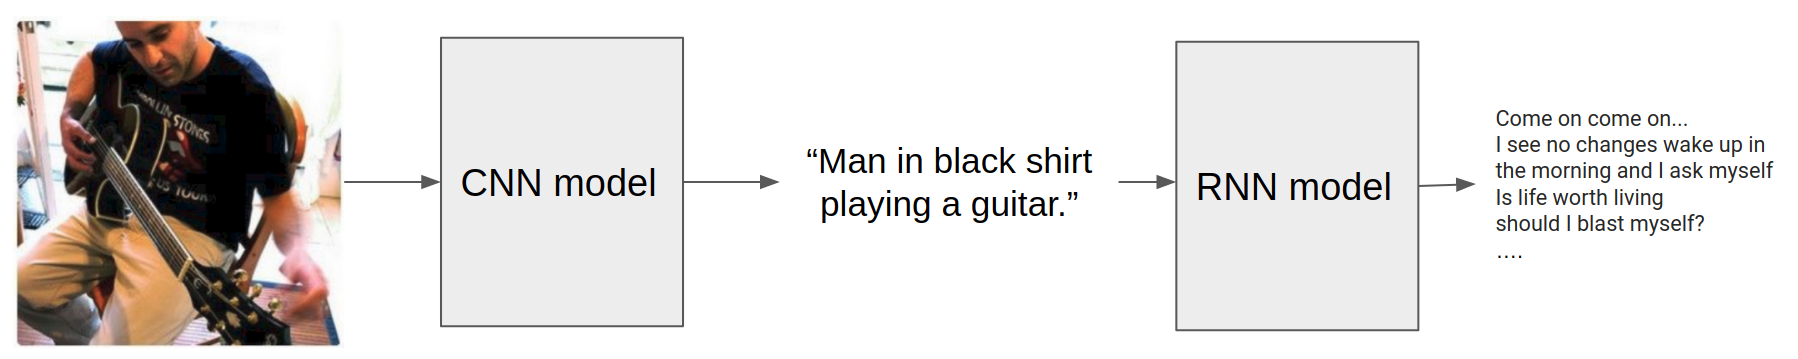
\includegraphics[scale=0.18]{figure1}
\caption{Architecture of the proposed implementation}
\label{fig:architecture}
\end{figure}

\end{document}
